\documentclass{school-22.101-notes}
\date{September 28, 2011}

\begin{document}
\maketitle



%%%%%%%%%%%%%%%%%%%%%%%% Infinite Square Well %%%%%%%%%%%%%%
\topic{Infinite Square Well/1D Particle In Box}\label{infinite-square-well}
This is an energy eigenvalue problem. We are given a box with the potential:
  \eqn{ V(x) = \left\{ \begin{array}{cc} 0 & 0 \le x \le L \\ \infty & x<0, x>L  \end{array} \right. }
  So there are infinite potential walls at location x=0 and x=L. Then we can immediately know the boundary conditions should be: $\psi_n (0) = 0, \psi_n(L) = 0$. 

  \textbf{Answer:} We divide the problem into two parts:
  \begin{enumerate}
  \item Outside: 
    \eqn{ \hat{H} = \frac{\hat{p}^2}{2m} + V = \infty }
  \item Inside: 
    \eqn{ \hat{H} = \frac{\hat{p}^2}{2m} + V = \frac{\hat{p}^2}{2m} }
    \eqn{ -\frac{\hbar^2}{2m} \ppxn2 \psi_n = E_n \psi_n \Rightarrow \ppxn2 \psi_n + k^2 \psi_n = 0 }
    Two BCs: $\psi_n (0) = \psi_n(L) =0$. 
    
    The solution is in the form of $\psi_n (x) = A \sin kx + B \cos kx$, apply BCs, we get $B=0, k_n = \frac{n \pi}{L} $. Now that we have constrain for k values, then the energy values are discrete/quantized as well: 
    \eqn{ E_n = \frac{\hbar^2 k^2_n}{2m} = \frac{\hbar^2 \pi^2 n^2}{2 m L^2} = n^2 \cdot E_1  }
    This has nothing to do with the quantum mechanical law itself -- it is really just the BC imposed that require the system to be discrete and quantized. 
    
    Then we find A through normalization process:
    \eqn{ \int_0^L A^2 \sin^2 (k_n x) = 1 \Rightarrow A = \sqrt{\frac{2}{L}} }
    \eqn{ \psi_n = \sqrt{\frac{2}{L}} \sin (k_n x)  }
    
  
\item \textbf{Interpretation:} There is a minimum energy related to the dimension of the box (the narrower the box, the higher the energy needs to be). The next possible states are: $4E_1, 9E_2,$ etc. For each energy, we are also able to define the state function as in Figure~\ref{particle-in-box}.
  \begin{figure}
    \centering
    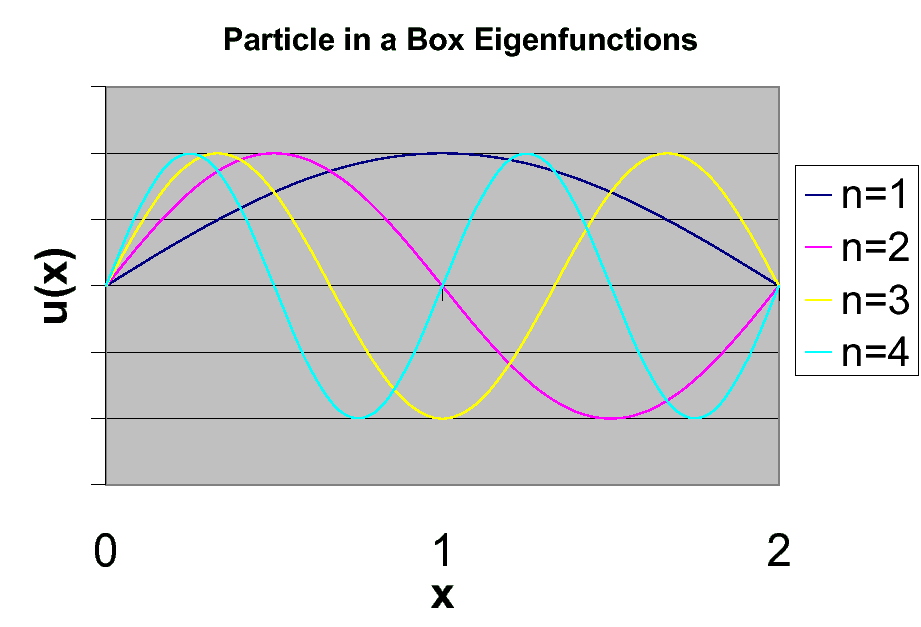
\includegraphics[width=4in]{images/qm/1Dparticle-in-box.png}
    \caption{Particle in Box Wave Function\label{particle-in-box}}
  \end{figure}
\end{enumerate}

%%%%%%%%%%%%%%%%%%%% FSW %%%%%%%%%%%%%%%%%%%%%%%%%%%
\topic{Finite Square Well}\label{finite-square-well}
This potential admits both bound states (with $E < 0$) and scattering states (with $E>0$). We will look at the bound states only\footnote{See Liboff 8.1, Krane 2.3 for more details}. We didn't really do this in class, but I just want to add a word: If we work out the scattering case of FSW, it turns out the transmission probability is sort of oscillating with respect of $E$, and the energies for perfect transmission turn out to precisely the allowed energies for the infinite square well \footnote{See Griffiths p79-82.}:
\eqn{ E_n + V_0 = \frac{n^2 \pi^2 \hbar^2}{2 m (2a)^2} }
\begin{figure}[ht]
    \centering
    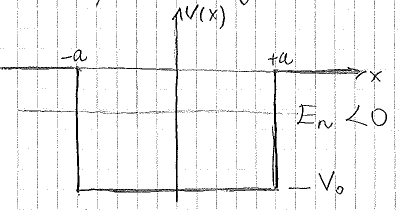
\includegraphics[width=3.5in]{images/qm/FSW.png}
    \caption{Finite Square Well Diagram}
\end{figure}

\uline{Intuitively}, we know:
\begin{itemize}
\item Inside the well, $KE = E_n - (-V_0) = E_n + V_0 > 0$, hence oscillatory wave. 
\item Outside the well, $KE = E_n - 0 = E_n <0$, hence finite propagation, analogous to the penetration we had in rectangular barrier before. When the energy is negative, instead of having $A e^{ikx} + B e^{-ikx}$ terms, we have $C e^{\kappa x} + D e^{-\kappa x}$ in which $\kappa$ is positive. 
\end{itemize}

%%%%%%%%%%%%%% Re-write Eqns %%%%%%%%%%%%
\subtopic{Re-write Schrodinger Equations}
\begin{align}
\hat{H} \psi_n(x)  = E_n \psi_n (x)  \Rightarrow - \frac{\hbar^2}{2m }   \dpsidxn2 + V(x) \psi_n (x) = E_n \psi_n (x) \\
\left\{ 
\begin{array}{ccc}
|x| < a:  & - \frac{\hbar^2}{2m } \dpsidxn2  -  (V_0 + E_n) \psi_n (x) = 0 & \Rightarrow \dpsidxn2 + k^2 \psi_n (x) = 0 \\
|x| > a:  & - \frac{\hbar^2}{2m } \dpsidxn2  -  E_n \psi_n (x) = 0         & \Rightarrow \dpsidxn2 - \kappa^2 \psi_n (x) = 0 
\end{array}
\right.
\end{align}
where
\eqn{ k = \sqrt{\frac{2m (V_0 + E_n)}{\hbar^2}} >0; \fsp \fsp \kappa = \sqrt{-\frac{2m E_n}{\hbar^2}} > 0 } 
Solution forms:
\begin{itemize}
\item BC: bounded states $ \Rightarrow |\psi (x \to \pm \infty)|^2 \to 0 \Rightarrow$ outside of the well, $\psi_{\mathrm{left}} (x) = C e^{\kappa x}, \psi_{\mathrm{right}} (x) = D e^{-\kappa x}$. 

\item Inside the FSW, we re-write $A^{\prime} e^{ikx} + B^{\prime} e^{-ikx} = A \sin (kx) + B \cos(kx)$ for reasons that would become clear in the parity section. 
\end{itemize}

\subtopic{Defined Parity}
Energy eigenfunctions in a symmetric position have a \textbf{`defined parity'} that is either odd or even in x. Definition of parity: $\sin(kx)$ is an odd parity because $\sin k(-x) = - \sin kx$. $\cos (kx)$ is an even parity because $\cos k(-x) = \cos kx$. 


%%%%%%%%%%%%% Odd Parity %%%%%%%%%%%%%%%%%%%%%%%
\subsubtopic{Odd Parity Solution (physical solution)}
\begin{enumerate}
\item \uline{Apply Boundary Conditions}
The BCs are: $\psi(a^+) = \psi(a^-), \psi^{\prime}(a^+) = \psi^{\prime}(a^-)$: 
\begin{align}
A \sin (ka) &= D e^{-\kappa a } \\
A k \cos (ka) &= - D \kappa e^{-\kappa a} = - \kappa A \sin (ka) \\
\Rightarrow \kappa &= - k \cot (ka)\label{BC}
\end{align}
Since $k = \sqrt{ \frac{2 m (V_0 + E)}{\hbar^2} }$, this is implying that there is certain constraint on E (as we hinted earlier that E should be in the form of $E_n$), both in term of the range, also in term of the permitted values. 

\item \uline{Define Potential Well Strength $\Lambda$: } Let's define $\Lambda$ as $-\alpha \cot \alpha = \sqrt{\Lambda^2 - \alpha^2}$. Then,
\eqn{ k^2 a^2 + \kappa^2 a^2 = \frac{2m V_0 a^2}{\hbar^2} = \Lambda^2 = \mbox{Strength of Potential Well} }
We call $\Lambda^2$ the strength of potential well, which depends on $V_0$ the depth of the well, and a the width of the well. 

\item \uline{Analytically Finding Constrains with Plots}
\begin{align}
\left.
\begin{array}{cc} 
\kappa^2 a^2 = \Lambda^2 - k^2 a^2  & \kappa a = \sqrt{\Lambda^2 - k^2 a^2} \\
Eq.\ref{BC} \times a                & \kappa a = - ka \cot (ka)
\end{array}
\right\}  \Rightarrow \boxed{ ka \cot (ka) = - \sqrt{ \Lambda^2 - k^2 a^2 } } 
\end{align}
If we consider $ka$ as the variable $x$, then the RHS is the bottom-right portion of a circle with $r = \Lambda$. The LHS is a $x \times \cot(x)$ curve that we can easily plot as well.
\begin{figure}[h!]
    \centering
    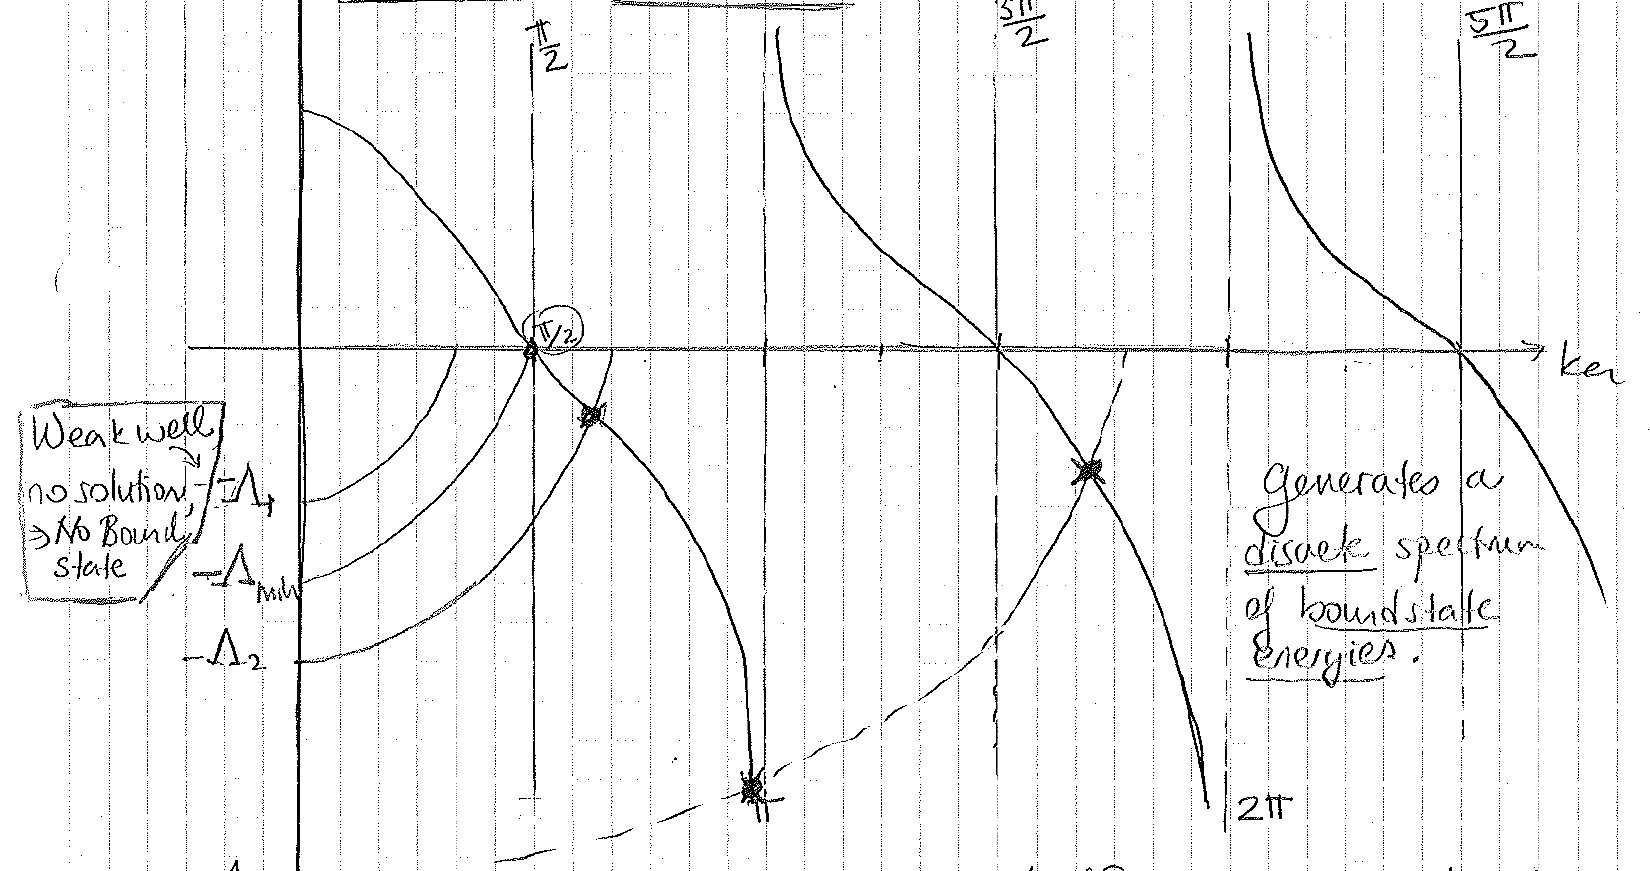
\includegraphics[width=4in]{images/qm/FSW-odd-graph-ka.png}
    \caption{Finite Square Well (Odd Parity), Constrains on $ka$\label{FSW-odd-graph-ka}}
\end{figure}

Interpretations of Figure~\ref{FSW-odd-graph-ka}: 
\begin{enumerate}
    \item Finite square well vs. Infinite square well:
    \begin{itemize}
    \item Similarity: BCs impose constrains on energies for both problems. 
    \item Difference: ISW's number of possible energy states is infinite (because the potential barrier is $\infty$!); FSW's strength $\Lambda^2$ limits the number of $E_n$ to be finite.  
    \end{itemize}
    
    \item \hi{Bound states mean $\Lambda \ge \frac{\pi}{2}$.} $\frac{\pi}{2}$ is the minimum $\Lambda$ value that allows any intersection. Wells weaker than $\frac{\pi}{2}$ would have no solution, that is, no bound state. 
     
    \item $\Lambda > \frac{\pi}{2}$  can be translated into constrains on $V_0$:
    \begin{align}
    \Lambda^2 &= \frac{2m V_0 a^2}{\hbar^2} > \frac{\pi^2}{4} \Rightarrow  
    \boxed{V_0 \ge \frac{\pi^2 \hbar^2}{8 m a^2} }
    \end{align}
    
    \item Number of bound states depends on $\Lambda$:
    \begin{align}
        \begin{dcases*}
         \frac{\pi}{2} < \Lambda < \frac{3\pi}{2}   & 1 solution \\
         \frac{3\pi}{2} < \Lambda < \frac{5 \pi}{2} & 2 solutions \\
         n \pi  - \frac{\pi}{2} < \Lambda < n \pi  + \frac{\pi}{2} & n solutions
        \end{dcases*}
    \end{align}
\end{enumerate}


\item \uline{Graphically Finding Constrains.} We can plot the $\sin$ curve inside the well, and notice that the $\sin$ wave inside the well must \textbf{`bend down'} on the boundary to match the decaying behavior outside the well. Effectively we are applying BCs graphically. 
\begin{figure}[h!]
    \centering
    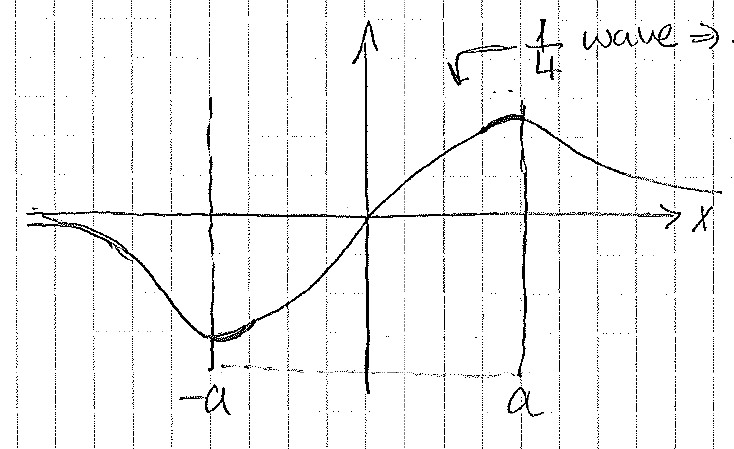
\includegraphics[width=4in]{images/qm/FSW-odd-graph-psi.png}
    \caption{Finite Square Well (Odd Parity), Graphically Finding Constrains} \label{FSW-odd-parity-graphically}
\end{figure}

Fig.~\ref{FSW-odd-parity-graphically} demonstrates the maximum wavelength condition, that is, 
\eqn{ \lambda = 4a \Rightarrow k = \frac{2 \pi}{\lambda} = \frac{\pi}{2a} }
Apply that bound state requires $E < 0 \Rightarrow 0 > E =  KE + V = |KE| - |V_0|, \Rightarrow |KE| <|V_0|$: 
\eqn{ V_0 > |KE| = \frac{\hbar^2 k^2}{2m} = \frac{\hbar^2 \pi^2}{8 ma^2} }
\end{enumerate}

%%%%%%%%%%%%%%%%%% Even Parity %%%%%%%%%%%%%%%%%%%%%%%%%%%%%%%%%%%%%%%%%%%%%%%%%
\subsubtopic{Even Parity Solution}
We essentially repeat what we did for the odd parity solutions but use $\cos(ka)$ instead of $\sin(ka)$ forms this time:
\begin{align}
A \cos (ka) &= D e^{-\kappa a} \\
-A k \sin (ka) &= - D \kappa e^{-\kappa a} = - A \kappa \cos (ka) \\
k \tan (ka) &= \kappa \\
ka \tan (ka) &= \kappa a = \sqrt{\Lambda^2 - k^2 a^2} 
\end{align}

\begin{figure}[h!]
    \centering
    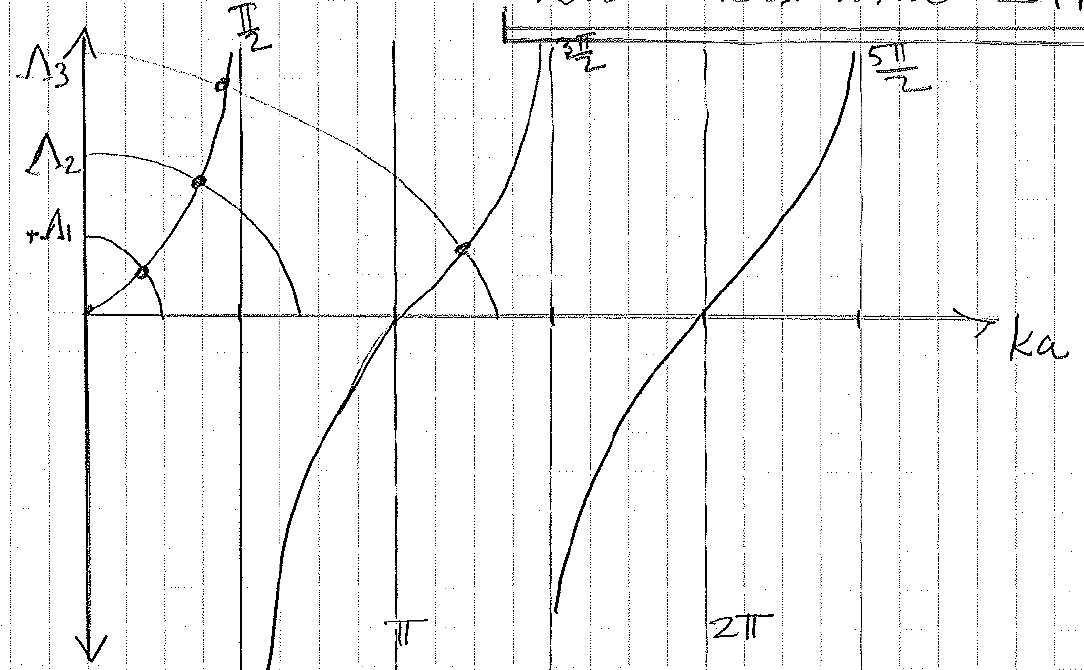
\includegraphics[width=3.7in]{images/qm/FSW-even-graph-ka.png}
    \caption{Finite Square Well(Even Parity), Constrains on $ka$}
    \label{FSW-even-graph-ka}
\end{figure}
\begin{figure}[h!]
    \centering
    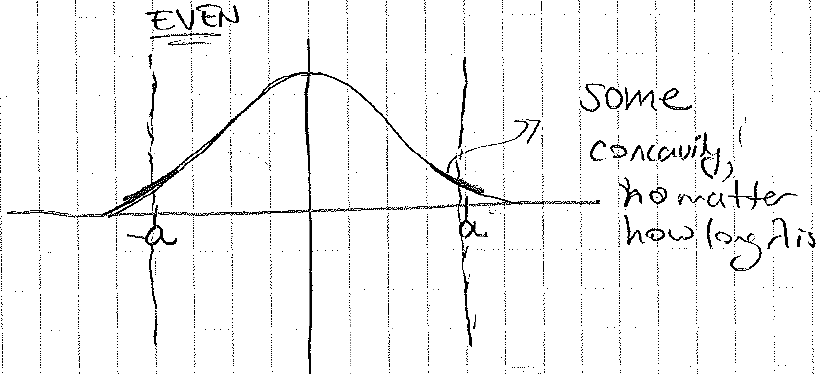
\includegraphics[width=4in]{images/qm/FSW-even-graph-psi.png}
    \caption{Finite Square Well (Even Parity), Graphically Finding Constrains}
    \label{FSW-even-graph-psi}
\end{figure}

\begin{itemize}
\item In Figure~\ref{FSW-even-graph-ka}, we plot the two sides of the constrain equation. In 1D regardless of the value of $\Lambda$ we always have at least one intersection. This implies that the even parity solution requires no bound state condition. 

\item In Figure~\ref{FSW-even-graph-psi}, we plot $\psi(x)$ vs. $x$, and notice that any $\cos(kx)$ can provide some concavity that let the out-of-the-well to be exponentially decaying. To put it differently, matching is possible no matter how long the wavelength is. KE can go to zero if needed to make BC work out. 

\item In reality, when we go to 3D, the odd solution will carry over, and the even solution will not be present. But for now just keep in mind that \textit{1D even solution has no bound state condition}. 
\end{itemize}

\end{document}
